\documentclass[12pt,aspectratio=169]{beamer}
% Shared Beamer setup for BIM Resilience biological-simulations decks.
% \input{} after \documentclass{beamer}.

\usetheme{Madrid}
\setbeamertemplate{navigation symbols}{}

\usepackage[T1]{fontenc}
\usepackage[utf8]{inputenc}
\usepackage{lmodern}
\usepackage{graphicx}
\usepackage{booktabs}
\usepackage{tikz}
\usetikzlibrary{arrows.meta,positioning,shapes.geometric,calc}
\usepackage{enumitem}
\setlist[itemize,1]{itemsep=2pt,topsep=2pt,parsep=0pt,partopsep=0pt,leftmargin=1.6em,label=\usebeamertemplate{itemize item}}
\setlist[itemize,2]{itemsep=1pt,topsep=1pt,parsep=0pt,partopsep=0pt,leftmargin=1.4em,label=\usebeamertemplate{itemize subitem}}
\setbeamerfont{normal text}{size=\normalsize}
\setbeamerfont{itemize/enumerate body}{size=\small}
\setbeamerfont{itemize/enumerate subbody}{size=\footnotesize}
\setbeamerfont{frametitle}{size=\Large,series=\bfseries}
\setbeamerfont{caption}{size=\footnotesize}
\usepackage{hyperref}
\hypersetup{colorlinks=true,linkcolor=,urlcolor=blue,citecolor=blue}

\definecolor{bimnavy}{HTML}{0F2A44}
\definecolor{bimnavylight}{HTML}{1B3A5C}
\definecolor{bimorange}{HTML}{C0410A}
\definecolor{bimsteel}{HTML}{4A7A9B}
\definecolor{bimcarry}{HTML}{0072B2}
\definecolor{bimreduce}{HTML}{E69F00}

\setbeamercolor{palette primary}{bg=bimnavy,fg=white}
\setbeamercolor{palette secondary}{bg=bimnavylight,fg=white}
\setbeamercolor{palette tertiary}{bg=bimsteel,fg=white}
\setbeamercolor{palette quaternary}{bg=bimnavy,fg=white}
\setbeamercolor{structure}{fg=bimorange}
\setbeamercolor{normal text}{fg=black,bg=white}
\setbeamercolor{background canvas}{bg=white}
\setbeamercolor{frametitle}{fg=white,bg=bimnavy}
\setbeamercolor{title}{fg=white,bg=bimnavy}
\setbeamercolor{section in head/foot}{fg=white,bg=bimnavy}
\setbeamercolor{subsection in head/foot}{fg=white,bg=bimsteel}
\setbeamercolor{author in head/foot}{fg=white,bg=bimnavy}
\setbeamercolor{title in head/foot}{fg=white,bg=bimnavy}
\setbeamercolor{date in head/foot}{fg=white,bg=bimnavy}
\setbeamercolor{page number in head/foot}{fg=bimnavy}
\setbeamercolor{block title}{fg=white,bg=bimorange}
\setbeamercolor{block body}{fg=black,bg=bimorange!8}
\setbeamercolor{item}{fg=bimorange}
\setbeamercolor{itemize item}{fg=bimorange}
\setbeamercolor{itemize subitem}{fg=bimsteel}
\setbeamercolor{alerted text}{fg=bimorange}
\setbeamertemplate{footline}[frame number]

\graphicspath{{./}}
\newcommand{\beamfig}[1]{%
  \includegraphics[width=\linewidth,height=0.58\textheight,keepaspectratio]{#1}}
\newcommand{\beamfigbig}[1]{%
  \includegraphics[width=\linewidth,height=0.74\textheight,keepaspectratio]{#1}}
\newcommand{\figcap}[1]{{\footnotesize\textcolor{bimsteel}{#1}}}

% Title slide: optional second argument is an orange eyebrow (e.g. ``10 minutes'').
\newcommand{\bimtitleslide}[2][]{%
  \begin{frame}[plain]
    \begin{tikzpicture}[remember picture, overlay]
      \fill[bimnavy] (current page.south west) rectangle (current page.north east);
      \node[regular polygon, regular polygon sides=6, minimum size=2.6cm,
            fill=bimorange, fill opacity=0.35, anchor=center, rotate=10]
        at ($(current page.south east)+(-1.6cm,1.3cm)$) {};
      \node[regular polygon, regular polygon sides=6, minimum size=2.0cm,
            fill=bimsteel, fill opacity=0.45, anchor=center, rotate=10]
        at ($(current page.south east)+(-3.4cm,2.1cm)$) {};
      \node[regular polygon, regular polygon sides=6, minimum size=1.4cm,
            fill=bimsteel, fill opacity=0.3, anchor=center, rotate=10]
        at ($(current page.south east)+(-1.0cm,3.1cm)$) {};
      \draw[bimorange, line width=2.4pt]
        ($(current page.west)+(2.1cm,1.9cm)$) -- ++(0,-3.3cm);
      \if\relax\detokenize{#1}\relax\else
        \node[anchor=west, font=\small\bfseries, text=bimorange!90!white]
          at ($(current page.west)+(2.7cm,1.55cm)$) {#1};
      \fi
      \node[anchor=west, text width=10.8cm, align=left, font=\Huge\bfseries, text=white]
        at ($(current page.west)+(2.7cm,1.05cm)$) {Biological Simulations};
      \node[anchor=west, text width=10.8cm, align=left, font=\Large, text=white]
        at ($(current page.west)+(2.7cm,0.35cm)$) {Stocks, Advice, and Scenarios};
      \node[anchor=west, text width=10.4cm, align=left, font=\normalsize, text=bimorange!85!white]
        at ($(current page.west)+(2.7cm,-0.5cm)$) {#2};
      \node[anchor=west, font=\small, text=white!85!bimnavy]
        at ($(current page.west)+(2.7cm,-1.75cm)$)
        {Laurence T. Kell \quad\textbullet\quad BIM Resilience Project \quad\textbullet\quad \today};
    \end{tikzpicture}
  \end{frame}}


\title[BIM Resilience --- 10 min]{Biological Simulations: Stocks, Advice, and Scenarios}
\subtitle{10-minute deck --- advice, what-ifs, mackerel example, CREST}
\author{Laurence T. Kell}
\institute{BIM Resilience Project}
\date{\today}

\begin{document}

\bimtitleslide[10 minutes]{Advice, scenarios, and how CREST turns them into a resilience tool}

% ------------------------------------------------------------
\begin{frame}{The thread (10 minutes)}
  \begin{itemize}
    \item \textbf{Advice} is conditioned on the \emph{past} --- and can flip at a benchmark
    \item \textbf{Scenarios} ask ``what if?'' under fixed fishing --- productivity, shocks, noise
    \item \textbf{CREST} carries those biological trajectories through to fleet value, effort and profit
  \end{itemize}
  \vspace{4mm}
  {\footnotesize\textcolor{bimsteel}{Resilience means being ready for flips --- the future will not be like the past.}}
\end{frame}

\begin{frame}{Resilience in a Changing World}
  \footnotesize
  \begin{itemize}
    \item \textbf{Can't Bounce Back} --- productivity and hence reference points are \emph{changing}
    \item \textbf{Stay Viable} --- not restore an equilibrium
  \end{itemize}
  \vspace{2mm}
  \begin{columns}[T]
    \begin{column}{0.48\textwidth}
      \textbf{Why it matters}
      \begin{itemize}
        \item Past strategies can fail under new regimes
        \item Fisheries: shifting productivity, distribution, recruitment, ...
      \end{itemize}
    \end{column}
    \begin{column}{0.48\textwidth}
      \textbf{What resilience means}
      \begin{itemize}
        \item \textbf{Persist} --- keep functioning
        \item \textbf{Adapt} --- change with conditions
        \item \textbf{Transform} --- change the system when needed
      \end{itemize}
    \end{column}
  \end{columns}
\end{frame}

% ------------------------------------------------------------
\begin{frame}{1. Advice --- status vs $B_{\mathrm{trigger}}$}
  \begin{columns}[T]
    \begin{column}{0.32\textwidth}
      \footnotesize
      Trend and reference points:
      \vspace{1mm}
      \begin{itemize}
        \item $\mathrm{SSB}/B_{\mathrm{trigger}}=1$?
        \begin{itemize}
          \item \textcolor{bimcarry}{$> 1$ --- carry on}
          \item \textcolor{bimreduce}{$<{ }1$ --- reduce $F$, catch, effort}
        \end{itemize}
        \item Crossing the line flips status and advice
        \item A benchmark can change $B_{\mathrm{trigger}}$
      \end{itemize}
    \end{column}
    \begin{column}{0.64\textwidth}
      \centering
      \beamfigbig{fig3.png}\\
      \figcap{$\mathrm{SSB}/B_{\mathrm{trigger}}$ --- blue above 1, orange below}
    \end{column}
  \end{columns}
\end{frame}

% ------------------------------------------------------------
\begin{frame}{2. Scenarios --- ``What Ifs''}
  \begin{columns}[T]
    \begin{column}{0.42\textwidth}
      \footnotesize
      \begin{itemize}
        \item Fixed fishing effort; examples not advice
        \item Status-quo; recruitment?
        \item Compare \emph{within} a stock: the gap is the assumption that changed
        \item \textbf{Resilience}: under current fishing, does catch get better, hold, or erode?
      \end{itemize}
    \end{column}
    \begin{column}{0.54\textwidth}
      \centering
      \beamfig{fig4.png}\\
      \figcap{Pelagics --- projected catch by scenario}
    \end{column}
  \end{columns}
\end{frame}

% ------------------------------------------------------------
\begin{frame}{3. Mackerel --- Recruitment}
  \begin{columns}[T]
    \begin{column}{0.42\textwidth}
      \footnotesize
      Worked example at status-quo $F$:
      \vspace{1mm}
      \begin{itemize}
        \item Recruitment deviance $\times 1$, $0.75$, $0.5$, $0.25$
        \item If effort stays as now, how does \textbf{catch} look?
      \end{itemize}
    \end{column}
    \begin{column}{0.54\textwidth}
      \centering
      \beamfig{fig_mac_rec.png}\\
      \figcap{Catch under recruitment multipliers}
    \end{column}
  \end{columns}
\end{frame}

\begin{frame}{3. Mackerel --- One-off $M$ shock}
  \begin{columns}[T]
    \begin{column}{0.42\textwidth}
      \footnotesize
      \begin{itemize}
        \item Same status-quo $F$/Effort
        \item Natural mortality $\times 5$ in \textbf{one year} (2035)
        \item A pulse --- what a smooth forecast misses
      \end{itemize}
    \end{column}
    \begin{column}{0.54\textwidth}
      \centering
      \beamfig{fig_mac_mshock.png}\\
      \figcap{Catch: baseline vs $M\times 5$ in 2035}
    \end{column}
  \end{columns}
\end{frame}

% ------------------------------------------------------------
\begin{frame}{4. CREST --- not an answering machine}
  \begin{columns}[T]
    \begin{column}{0.52\textwidth}
      \footnotesize
      \textbf{CREST}: Capacity, Resilience and Economic Shock Transmission
      \vspace{1mm}
      \begin{itemize}
        \item Industry asks \emph{``what if \ldots?''}
        \item Is the fleet resilient --- or should it be?
        \item Biological shocks $\rightarrow$ value, effort, profit
        \item Between stock assessment and a whole-economy model
      \end{itemize}
    \end{column}
    \begin{column}{0.44\textwidth}
      \centering
      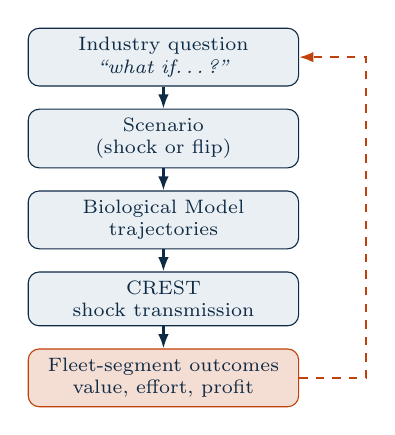
\begin{tikzpicture}[
          node distance=2.8mm and 3mm,
          box/.style={draw=bimnavy, rounded corners, fill=bimsteel!12,
                      align=center, minimum height=5.5mm, text width=3.2cm,
                      font=\scriptsize, text=bimnavy},
          outbox/.style={box, fill=bimorange!18, draw=bimorange},
          arr/.style={-{Latex[length=1.8mm]}, thick, bimnavy}
        ]
        \node[box] (q) {Industry question\\\emph{``what if\dots?''}};
        \node[box, below=of q] (s) {Scenario \\ (shock or flip)};
        \node[box, below=of s] (bm) {Biological Model \\ trajectories};
        \node[box, below=of bm] (crest) {CREST \\ shock transmission};
        \node[outbox, below=of crest] (out) {Fleet-segment outcomes \\ value, effort, profit};
        \draw[arr] (q) -- (s);
        \draw[arr] (s) -- (bm);
        \draw[arr] (bm) -- (crest);
        \draw[arr] (crest) -- (out);
        \draw[arr, dashed, bimorange] (out.east) -- ++(0.85,0) |- (q.east);
      \end{tikzpicture}
    \end{column}
  \end{columns}
\end{frame}

% ------------------------------------------------------------
\begin{frame}{Takeaways}
  \begin{itemize}
    \item Advice is based on the past --- benchmarks can reclassify status
    \item Scenarios probed the future under advice rule --- recruitment, shocks, noise
    \item Mackerel shows how catch responds to productivity and one-off flips
    \item CREST allows the fleet to ask the question
  \end{itemize}
  \vspace{4mm}
  {\footnotesize\textcolor{bimsteel}{Full deck: \texttt{biological\_simulations\_slides.pdf}}}
\end{frame}

\end{document}
